\newcommand{\titulus}{\nomenFesti{Dominica infra Octavam Ss. Petri et Pauli.}
\celebratio{Semiduplex.}}
\newcommand{\dominica}{Dominica}
\newcommand{\festumveldominica}{Dominica}
\newcommand{\solemnis}{Dominica}
\newcommand{\lectioi}{\pars{Lectio I.} \scriptura{2 Reg. 1, 1-4}

\noindent Incipit liber secúndus Regum.

\noindent Factum est autem, postquam mórtuus est Saul, ut David reverterétur a cæde Amalec et manéret in Síceleg duos dies. In die autem tértia appáruit homo véniens de castris Saul veste conscíssa et púlvere conspérsus caput et, ut venit ad David, cécidit super fáciem suam et adorávit. Dixítque ad eum David: Unde venis? Qui ait ad eum: De castris Israël fugi. Et dixit ad eum David: Quod est verbum quod factum est? Indica mihi. Qui ait: Fugit pópulus ex prǽlio, et multi corruéntes e pópulo mórtui sunt; sed et Saul et Iónathas fílius eius interiérunt.}
\newcommand{\lectioii}{\pars{Lectio II.} \scriptura{2 Reg. 1, 5-10}

\noindent Dixítque David ad adolescéntem qui nuntiábat ei: Unde scis quia mórtuus est Saul et Iónathas fílius eius? Et ait adoléscens qui nuntiábat ei: Casu veni in montem Gélboë, et Saul incumbébat super hastam suam. Porro currus et équites appropinquábant ei, et convérsus post tergum suum vidénsque me vocávit; cui cum respondíssem: Adsum, dixit mihi: Quisnam es tu? Et aio ad eum: Amalecítes ego sum. Et locútus est mihi: Sta super me et intérfice me, quóniam tenent me angústiæ, et adhuc tota ánima mea in me est. Stansque super eum, occídi illum, sciébam enim quod vívere non póterat post ruínam; et tuli diadéma, quod erat in cápite eius et armíllam de brácchio illíus et áttuli ad te dóminum meum huc.}
\newcommand{\lectioiii}{\pars{Lectio III.} \scriptura{2 Reg. 1, 11-15}

\noindent Apprehéndens autem David, vestiménta sua scidit, omnésque viri, qui erant cum eo, et planxérunt, et flevérunt, et ieiunavérunt usque ad vésperam super Saul, et super Iónathan fílium eius, et super pópulum Dómini et super domum Israël, eo quod corruíssent gládio. Dixítque David ad iúvenem qui nuntiáverat ei: Unde es tu? Qui respóndit: Fílius hóminis ádvenæ Amalecítæ ego sum. Et ait ad eum David: Quare non timuísti míttere manum tuam, ut occíderes christum Dómini? Vocánsque David unum de púeris suis ait: Accédens írrue in eum. Qui percússit illum, et mórtuus est.}
\newcommand{\lectioiv}{\pars{Lectio IV.} \scriptura{Liber 4, Cap. 3 et 4}

\noindent Ex libro Morálium sancti Gregórii Papæ.

\noindent Quid est quod David, qui retribuéntibus sibi mala non réddidit, cum Saul et Iónathas bello occúmberent, Gélboë móntibus maledíxit, dicens: Montes Gélboë, nec ros nec plúvia véniant super vos: neque sint agri primitiárum: quia ibi abiéctus est clýpeus fórtius, clýpeus Saul, quasi non esset unctus óleo? Quid est quod Ieremías, cum prædicatiónem suam cérneret audiéntium difficultáte præpedíri, maledíxit dicens: Maledíctus vir, qui annuntiávit patri meo, dicens: Natus est tibi puer másculus?}
\newcommand{\lectiov}{\pars{Lectio V.}

\noindent Quid ergo montes Gélboë, Saul moriénte, deliquérunt, quátenus in eos nec ros nec plúvia cáderet et ab omni eos viriditátis gérmine senténtiæ sermo siccáret? Sed quia Gélboë interpretátur decúrsus, per Saul autem unctum et mórtuum mors nostri mediatóris exprímitur; non immérito per Gélboë montes supérba Iudæórum corda signántur, quæ dum in huius mundi desidériis défluunt, in Christi, id est, uncti se morte miscuérunt: et quia in eis unctus rex corporáliter móritur, ipsi ab omni grátiæ rore siccántur.}
\newcommand{\lectiovi}{\pars{Lectio VI.}

\noindent De quibus et bene dícitur, ut agri primitiárum esse non possint. Supérbæ quippe Hebræórum mentes primitívos fructus non ferunt: quia in Redemptóris advéntu ex parte máxima in perfídia remanéntes, primórdia fídei sequi noluérunt. Sancta namque Ecclésia in primítiis suis multitúdine Géntium fœcundáta, vix in mundi fine Iudǽos quos invénerit, súscipit, et extréma cólligens, eos quasi relíquias frugum ponit.}
\newcommand{\lectiovii}{\pars{Lectio VII.} \scriptura{Mt. 5, 20-24}

\noindent Léctio sancti Evangélii secúndum Matthǽum.

\noindent In illo témpore: Dixit Iesus discípulis suis: Nisi abundáverit iustítia vestra plus quam scribárum et pharisæórum, non intrábitis in regnum cælórum. Et réliqua.

\scriptura{Liber 1 de Sermóne Dómini in monte, cap. 9}

\noindent Homilía sancti Augustíni Epíscopi.

\noindent Iustítia pharisæórum est, ut non occídant: iustítia eórum, qui intratúri sunt in regnum cælórum, ut non irascántur sine causa. Mínimum est ergo, non occídere; et qui illud sólverit, mínimus vocábitur in regno cælórum. Qui autem illud impléverit, ut non occídat, non contínuo magnus erit, et idóneus regno cælórum; sed tamen ascéndit áliquem gradum: perficiétur autem, si nec irascátur sine causa; quod si perfécerit, multo remótior erit ab homicídio. Quaprópter qui docet ut non irascámur, non solvit legem ne occidámus, et in corde, dum non iráscimur, innocéntiam custodiámus.}
\newcommand{\lectioviii}{\pars{Lectio VIII.}

\noindent Gradus ítaque sunt in istis peccátis: ut primo quisque irascátur, et eum motum retíneat corde concéptum. Iam si extórserit vocem indignántis ipsa commótio, non significántem áliquid, sed illum ánimi motum ipsa eruptióne testántem, qua feriátur ille, cui iráscitur; plus est útique, quam si surgens ira siléntio premerétur. Si vero non solum vox indignántis audiátur, sed étiam verbum, quo iam certam eius vituperatiónem, in quem profértur, desígnet et notet; quis dúbitet, ámplius hoc esse, quam si solus indignatiónis sonus ederétur?}

\newcommand{\lectioix}{\pars{Lectio IX.}

\noindent Vide nunc étiam tres reátus, iudícii, concílii, et gehénnæ ignis. Nam in iudício adhuc defensióni datur locus. In concílio autem, quamquam et iudícium esse sóleat, tamen quia interésse áliquid hoc loco fatéri cogit ipsa distínctio, vidétur ad concílium pertinére senténtiæ prolátio; quando non iam cum ipso reo ágitur, utrum damnándus sit; sed inter se, qui iúdicant, cónferunt quo supplício damnári opórteat, quem constat esse damnándum. Gehénna vero ignis, nec damnatiónem habet dúbiam, sicut iudícium, nec damnáti pœnam, sicut concílium: in gehénna quippe ignis, certa est damnátio, et pœna damnáti.}
% LuaLaTeX

\documentclass[a4paper, twoside, 12pt]{article}
\usepackage[latin]{babel}
%\usepackage[landscape, left=3cm, right=1.5cm, top=2cm, bottom=1cm]{geometry} % okraje stranky
%\usepackage[landscape, a4paper, mag=1166, truedimen, left=2cm, right=1.5cm, top=1.6cm, bottom=0.95cm]{geometry} % okraje stranky
\usepackage[landscape, a4paper, mag=1400, truedimen, left=0.5cm, right=0.5cm, top=0.5cm, bottom=0.5cm]{geometry} % okraje stranky

\usepackage{fontspec}
\setmainfont[FeatureFile={junicode.fea}, Ligatures={Common, TeX}, RawFeature=+fixi]{Junicode}
%\setmainfont{Junicode}

% shortcut for Junicode without ligatures (for the Czech texts)
\newfontfamily\nlfont[FeatureFile={junicode.fea}, Ligatures={Common, TeX}, RawFeature=+fixi]{Junicode}

\usepackage{multicol}
\usepackage{color}
\usepackage{lettrine}
\usepackage{fancyhdr}

% usual packages loading:
\usepackage{luatextra}
\usepackage{graphicx} % support the \includegraphics command and options
\usepackage{gregoriotex} % for gregorio score inclusion
\usepackage{gregoriosyms}
\usepackage{wrapfig} % figures wrapped by the text
\usepackage{parcolumns}
\usepackage[contents={},opacity=1,scale=1,color=black]{background}
\usepackage{tikzpagenodes}
\usepackage{calc}
\usepackage{longtable}
\usetikzlibrary{calc}

\setlength{\headheight}{14.5pt}

% Commands used to produce a typical "Conventus" booklet

\newenvironment{titulusOfficii}{\begin{center}}{\end{center}}
\newcommand{\dies}[1]{#1

}
\newcommand{\nomenFesti}[1]{\textbf{\Large #1}

}
\newcommand{\celebratio}[1]{#1

}

\newcommand{\hora}[1]{%
\vspace{0.5cm}{\large \textbf{#1}}

\fancyhead[LE]{\thepage\ / #1}
\fancyhead[RO]{#1 / \thepage}
\addcontentsline{toc}{subsection}{#1}
}

% larger unit than a hora
\newcommand{\divisio}[1]{%
\begin{center}
{\Large \textsc{#1}}
\end{center}
\fancyhead[CO,CE]{#1}
\addcontentsline{toc}{section}{#1}
}

% a part of a hora, larger than pars
\newcommand{\subhora}[1]{
\begin{center}
{\large \textit{#1}}
\end{center}
%\fancyhead[CO,CE]{#1}
\addcontentsline{toc}{subsubsection}{#1}
}

% rubricated inline text
\newcommand{\rubricatum}[1]{\textit{#1}}

% standalone rubric
\newcommand{\rubrica}[1]{\vspace{3mm}\rubricatum{#1}}

\newcommand{\notitia}[1]{\textcolor{red}{#1}}

\newcommand{\scriptura}[1]{\hfill \small\textit{#1}}

\newcommand{\translatioCantus}[1]{\vspace{1mm}%
{\noindent\footnotesize \nlfont{#1}}}

% pruznejsi varianta nasledujiciho - umoznuje nastavit sirku sloupce
% s prekladem
\newcommand{\psalmusEtTranslatioB}[3]{
  \vspace{0.5cm}
  \begin{parcolumns}[colwidths={2=#3}, nofirstindent=true]{2}
    \colchunk{
      \input{#1}
    }

    \colchunk{
      \vspace{-0.5cm}
      {\footnotesize \nlfont
        \input{#2}
      }
    }
  \end{parcolumns}
}

\newcommand{\psalmusEtTranslatio}[2]{
  \psalmusEtTranslatioB{#1}{#2}{8.5cm}
}


\newcommand{\canticumMagnificatEtTranslatio}[1]{
  \psalmusEtTranslatioB{#1}{temporalia/extra-adventum-vespers/magnificat-boh.tex}{12cm}
}
\newcommand{\canticumBenedictusEtTranslatio}[1]{
  \psalmusEtTranslatioB{#1}{temporalia/extra-adventum-laudes/benedictus-boh.tex}{10.5cm}
}

% volne misto nad antifonami, kam si zpevaci dokresli neumy
\newcommand{\hicSuntNeumae}{\vspace{0.5cm}}

% prepinani mista mezi notovymi osnovami: pro neumovane a neneumovane zpevy
\newcommand{\cantusCumNeumis}{
  \setgrefactor{17}
  \global\advance\grespaceabovelines by 5mm%
}
\newcommand{\cantusSineNeumas}{
  \setgrefactor{17}
  \global\advance\grespaceabovelines by -5mm%
}

% znaky k umisteni nad inicialu zpevu
\newcommand{\superInitialam}[1]{\gresetfirstlineaboveinitial{\small {\textbf{#1}}}{\small {\textbf{#1}}}}

% pars officii, i.e. "oratio", ...
\newcommand{\pars}[1]{\textbf{#1}}

\newenvironment{psalmus}{
  \setlength{\parindent}{0pt}
  \setlength{\parskip}{5pt}
}{
  \setlength{\parindent}{10pt}
  \setlength{\parskip}{10pt}
}

%%%% Prejmenovat na latinske:
\newcommand{\nadpisZalmu}[1]{
  \hspace{2cm}\textbf{#1}\vspace{2mm}%
  \nopagebreak%

}

% mode, score, translation
\newcommand{\antiphona}[3]{%
\hicSuntNeumae
\superInitialam{#1}
\includescore{#2}

#3
}
 % Often used macros
%%%% Preklady jednotlivych zpevu (nektere se opakuji, a je dobre mit je
% vsechny na jedne hromade)

\newcommand{\trOratioAnteOfficium}{\translatioCantus{Otevři, Pane, má ústa, abych chválil tvé svaté jméno.
Očisti mé srdce od všech marnivých, zvrácených a~jiných myšlenek, osvěť rozum, rozněť cit,
abych mohl důstojně, soustředěně a~zbožně recitovat a~vysloužil si být
vyslyšen před tváří tvé velebnosti. Skrze Krista…}}

\newcommand{\trOratioPostOfficium}{\translatioCantus{\textit{Následující modlitbu
opatřil pro ty, kdo ji zbožně vyřknou po hodinkách, zesnulý papež Lev X.
odpustky za hříchy vzniklé při konání hodinek z~lidské křehkosti. Říká se
vkleče.}
Svatosvaté a~nerozdílné Trojici, ukřižovanému lidství našeho Pána Ježíše
Krista, přeblažené a~přeslavné plodné neporušenosti vždy Panny Marie
i~souhrnu všech svatých buď ode všeho stvoření věčná chvála, čest a~sláva, nám
pak buď dáno odpuštění všech hříchů, po nekonečné věky věků. Amen.}}

% HOURS ---

\newcommand{\trAntI}{\translatioCantus{Jasné narození slavné Panny Marie,
z pokolení (dosl. ze semene) Abrahámova, vzešlé z kmene Judova, z rodu Davidova.}}
\newcommand{\trAntII}{\translatioCantus{Dnes je Narození svaté Panny 
Marie, jejíž předrahý život osvěcuje všechny církve.}}

\newcommand{\trAntIII}{\translatioCantus{Maria, jež vzešla 
z královského rodu, září; myslí i duchem ji zbožně prosíme, aby 
nám pomáhala svými přímluvami.}}

\newcommand{\trAntIV}{\translatioCantus{Srdcem i duchem pějme Kristu 
k slávě o této svaté slavnosti vznešené Rodičky Boží Marie.}}

\newcommand{\trAntV}{\translatioCantus{Příjemně \notitia{?} 
oslavujme Narození blahoslavené Marie,
aby se ona za nás přimlouvala u Pána Ježíše Krista.}}

\newcommand{\trCapituli}{\translatioCantus{Před věky, na počátku mě stvořil, potrvám věčně. Ve svatém Stanu jsem před ním konala službu.}}

\newcommand{\trRespVesp}{\translatioCantus{Buď zdráva, Maria,
plná milosti: \grestar{} Pán s tebou. \Vbardot{} Požehnaná jsi mezi ženami,
a požehnaný plod života (ve smyslu lůna, břicha) tvého.}}

\newcommand{\trVersus}{\translatioCantus{\Vbardot{} Dnes je Narození svaté Panny Marie. \Rbardot{} Jejíž předrahý život osvěcuje všechny církve.}}

\newcommand{\trAntMagnificatI}{\translatioCantus{Konejme památku
veledůstojného narození slavné Panny Marie,
jíž se dostalo mateřské důstojnosti bez ztráty panenské cudnosti.}}

% Tento preklad je vice nez nejisty a ani alternativy, ktere jsem
% videl, me nepresvedcily...
\newcommand{\trAntBenedictus}{\translatioCantus{Slavnostně slavme 
dnešní narození Marie, vždy Panny a Rodičky Boží: v něm se objevuje
vysokost trůnu (totiž Marie, trůnu Božího Syna), aleluja.}}

\newcommand{\trAntMagnificatII}{\translatioCantus{Tvé narození,
Bohorodičko Panno, vyhlásilo radost celému světu:
z tebe totiž vzešlo Slunce spravedlnosti, Kristus, náš Bůh:
jenž zrušil kletbu a dal nám požehnání: přemohl smrt a dal nám život věčný.}}

\newcommand{\trOrationis}{\translatioCantus{Prosíme tě, Bože, 
uděl svým služebníkům dar nebeské milosti,
aby těm, jimž slehnutím blahoslavené Panny vyvstal počátek spásy, 
slavnost k poctě jejího narození přinesla
rozhojnění pokoje.
Skrze tvého Syna, našeho Pána Ježíše Krista, který s tebou žije a kraluje,
Bůh, v jednotě Ducha svatého po všechny věky věků.}}

\newcommand{\trFideliumAnimae}{\translatioCantus{\Vbardot{} Duše věrných ať pro
milosrdenství Boží odpočívají v~pokoji. \Rbardot{} Amen.}}

% Completorium

\newcommand{\trJubeDomne}{\translatioCantus{Rač, pane, požehnat.}}

\newcommand{\trComplBenedictio}{\translatioCantus{Pokojnou noc a~svatou smrt
nechť nám dopřeje všemohoucí Pán. \Rbardot{} Amen.}}

\newcommand{\trComplLectioBr}{\translatioCantus{Buďte střízliví, bděte.
Váš protivník Ďábel obchází jako lev řvoucí a~hledá, koho by pohltil.
Postavte se proti němu pevní ve víře.  Ale ty, Pane, smiluj se nad námi.
\Rbardot{} Bohu díky.}}

\newcommand{\trComplAntI}{\translatioCantus{Rač se smilovati nade mnou,
Hospodine, a vyslyš mou modlitbu.}}

\newcommand{\trComplCapituli}{\translatioCantus{Jsi přece, Hospodine,
uprostřed nás a~jmenujeme se po tobě.  Neopouštěj nás, Pane, náš Bože.}}

\newcommand{\trRespCompl}{\translatioCantus{Do tvých rukou, Pane, \grestar{}
poroučím svého ducha. \Vbardot{} Ty mne zachráníš, Pane, Bože věrný.}}

\newcommand{\trComplVersus}{\translatioCantus{\Vbardot{} Střez mne jako zřítelnici oka,
aleluja. \Rbardot{} Ve stínu svých křídel uschovej mne, aleluja.}}

\newcommand{\trAntSalvaNos}{\translatioCantus{Ochraňuj nás, Pane, když
bdíme, a~buď s~námi, když spíme, ať bdíme s~Kristem a~odpočíváme v~pokoji.}}

\newcommand{\trComplOrationis}{\translatioCantus{Zavítej, prosíme, Pane, sem
do našeho příbytku a~daleko od něj zažeň všechny úklady nepřítele. Ať tu
bydlí tví svatí andělé a~tvoje požehnání buď nad ním stále. Skrze…}}

\newcommand{\trSalveRegina}{\translatioCantus{Zdrávas Královno, matko
milosrdenství, živote, sladkosti a naděje naše, buď zdráva!
K tobě voláme, vyhnaní synové Evy,
k tobě vzdycháme, lkajíce a plačíce
v tomto slzavém údolí.
A proto, orodovnice naše,
obrať k nám své milosrdné oči
a Ježíše, požehnaný plod života svého,
nám po tomto putování ukaž,
ó milostivá, ó přívětivá,
ó přesladká, Panno Maria!}}

\newcommand{\trOraProNobis}{\translatioCantus{\Vbardot{} 
Oroduj za nás, svatá Boží Rodičko,
\Rbardot{} aby nám Kristus dal účast na svých zaslíbeních.}}

% Matutinum

\newcommand{\trMatInvitatorium}{\translatioCantus{}}

\newcommand{\trMatVeniteA}{\translatioCantus{Pojďte, chvalme s~radostí Pána,
s~jásotem slavme Boha, svou spásu; předstupme před tvář jeho s~díky, písně plesu pějme jemu.}}

\newcommand{\trMatVeniteB}{\translatioCantus{Neboť Bůh veliký jest Hospodin, a~král nade všecky bohy.
Jsouť v~jeho ruce všecky hlubiny země, temena hor jsou majetek jeho.}}

\newcommand{\trMatVeniteC}{\translatioCantus{Jehoť jest moře, neb on je učinil; i~souš
je dílo jeho rukou. Pojďme, klanějme se, padněme, klekněme před Pánem, svým
tvůrcem. Jeť on Pán, náš Bůh, a~my jsme lid, jejž on vodí a~ovce, jež pase.}}

\newcommand{\trMatVeniteD}{\translatioCantus{Kéž byste poslechli dnes hlasu jeho:
,,Nezatvrzujte svých srdcí jak v~Hádce, jak v~Pokušení na poušti, kde vaši otcové pokoušeli mne,
zkoušeli mne, ač vídali skutky mé.``}}

\newcommand{\trMatVeniteE}{\translatioCantus{Čtyřicet roků mrzel jsem se na to pokolení
a~řekl jsem: ,,Lid je to myslí stále bloudící``! Oni však nechtěli znáti mé cesty, takže jsem
přisáhl ve svém hněvu: ,,Nedojdou odpočinku mého!\mbox{}``}}

\newcommand{\trMatAntI}{\translatioCantus{}}

\newcommand{\trMatAntII}{\translatioCantus{}}

\newcommand{\trMatAntIII}{\translatioCantus{}}

\newcommand{\trMatVersusI}{\translatioCantus{}}

\newcommand{\trMatAbsolutioI}{\translatioCantus{Vyslyš Pane Ježíši Kriste
prosby svých služebníků \gredagger{} a~smiluj se nad námi, \grestar{} jenž
s~Otcem a~Duchem…}}

\newcommand{\trMatBenedictioI}{\translatioCantus{Rač, pane, požehnat.
Věčný Otec nám stále žehnej. \Rbardot{} Amen.}}

\newcommand{\trMatLecI}{\translatioCantus{Kéž by mě zulíbal polibky svých úst. 
Tvé milování je nad víno lahodnější;
vybraně voní tvé voňavky;
rozlévající se olej je tvé jméno,
proto tě dívky milují.
Strhni mě za sebou, poběžme!
Král mě uvedl do svých komnat;
budeš nám radostí a jásotem.
Víc než víno oslavíme tvé milování;
věru po právu jsi milován!
Snědá jsem, a přece krásná, jeruzalémské dcery,
jako stany kedarské,
jako šalmské závěsy.
}}

\newcommand{\trMatRespI}{\translatioCantus{}}

\newcommand{\trMatBenedictioII}{\translatioCantus{Rač, pane, požehnat.
Jednorozený Boží Syn nám žehnej \grestar{} a nám pomáhej. \Rbardot{} Amen.}}

\newcommand{\trMatLecII}{\translatioCantus{Nehleďte na mou osmahlou pleť:
to mě slunce ožehlo.
Synové mé matky se na mne rozzlobili,
poslali mě hlídat vinice.
A svou vinici, tu jsem nehlídala!
Pověz mi tedy, ty, jehož miluje mé srdce:
kam zavedeš své stádo pást,
kde ho necháš za poledne odpočívat?
Abych už nebloudila jako tulačka
poblíž stád druhů tvých.
Nevíš-li to, nejrásnější z žen,
jdi po stopách stáda
a kůzlata svá zaveď, ať se pasou
poblíž obydlí pastýřů.
Ke své klisně zapřažené do vozu faraonova
tebe, mé milá, přirovnávám.
Stále krásné jsou tvé líce s náušnicemi
i tvé hrdlo v náhrdelnících.}}

\newcommand{\trMatRespII}{\translatioCantus{}}

\newcommand{\trMatBenedictioIII}{\translatioCantus{Rač, pane, požehnat.
Milost Ducha Svatého ať osvítí nám smysly \grestar{} i srdce. \Rbardot{} Amen.}}

\newcommand{\trMatLecIII}{\translatioCantus{Zhotovíme ti zlaté náušnice
a kuličky ze stříbra.
Když král stoluje,
vydechuje můj nard svou vůni.
Můj milý je polštářek s myrhou,
jenž mi odpočívá mezi ňadry.
Můj milý je hrozen šáchoru
ve vinicích v Engadi.
Jak jsi krásná, milá moje,
jak jsi krásná!
Tvé oči jsou holubice.
Jak jsi krásný, můj milý,
jak líbezný!
Naše lože je samá zeleň.
Trámoví našeho domu je z cedru,
naše ostění z cypřiše.}}

\newcommand{\trMatRespIII}{\translatioCantus{}}

\newcommand{\trMatAntIV}{\translatioCantus{}}

\newcommand{\trMatAntV}{\translatioCantus{}}

\newcommand{\trMatAntVI}{\translatioCantus{}}

\newcommand{\trMatVersusII}{\translatioCantus{}}

\newcommand{\trMatAbsolutioII}{\translatioCantus{
Tvá milost a laskavost nechť nám pomáhá, jenž žiješ a vládneš s Otcem a Svatým Duchem na věky věků.}}

\newcommand{\trMatBenedictioIV}{\translatioCantus{Rač, pane, požehnat.
Bůh Otec všemohoucí, \grestar{} buď k nám milostivý a odpouštějící. \Rbardot{} Amen.}}

\newcommand{\trMatLecIV}{\translatioCantus{}}

\newcommand{\trMatRespIV}{\translatioCantus{}}

\newcommand{\trMatBenedictioV}{\translatioCantus{}}

\newcommand{\trMatLecV}{\translatioCantus{}}

\newcommand{\trMatRespV}{\translatioCantus{}}

\newcommand{\trMatBenedictioVI}{\translatioCantus{Rač, pane, požehnat.
Bůh rozněť v nás oheň své lásky. \Rbardot{} Amen.}}

\newcommand{\trMatLecVI}{\translatioCantus{}}

\newcommand{\trMatRespVI}{\translatioCantus{}}

\newcommand{\trMatAntVII}{\translatioCantus{}}

\newcommand{\trMatAntVIII}{\translatioCantus{}}

\newcommand{\trMatAntIX}{\translatioCantus{}}

\newcommand{\trMatVersusIII}{\translatioCantus{}}

\newcommand{\trMatAbsolutioIII}{\translatioCantus{Z okovů našich hříchů,
\grestar{} vysvoboď nás všemohoucí a milosrdný Pán. \Rbardot{} Amen.}}

\newcommand{\trMatBenedictioVII}{\translatioCantus{Rač, pane, požehnat.
Čtení evangelia nechť je nám \grestar{} spásou a ochranou. \Rbardot{} Amen.}}

\newcommand{\trMatLecVIIa}{\translatioCantus{
  Rodokmen Ježíše Krista, syna Davidova, syna Abrahámova:
  Abrahám zplodil Izáka,
  Izák zplodil Jakuba.}}

\newcommand{\trMatLecVIIb}{\translatioCantus{}}

\newcommand{\trMatRespVII}{\translatioCantus{}}

\newcommand{\trMatBenedictioVIII}{\translatioCantus{Rač, pane, požehnat.
\Rbardot{} Amen.}}

\newcommand{\trMatLecVIII}{\translatioCantus{}}

\newcommand{\trMatRespVIII}{\translatioCantus{}}

\newcommand{\trMatBenedictioIX}{\translatioCantus{Rač, pane, požehnat.
Do společnosti občanů nebes \grestar{} ať nás dovede král andělů.
\Rbardot{} Amen.}}

\newcommand{\trMatLecIX}{\translatioCantus{}}

% from the Czech Liturgia horarum
\newcommand{\trTeDeum}{\begin{translatioMulticol}{3}

Bože, tebe chválíme, 
tebe, Pane, velebíme.

Tebe, věčný Otče, 
oslavuje celá země.

Všichni andělé, 
cherubové i~serafové,

všechny mocné nebeské zástupy 
bez ustání volají:

Svatý, Svatý, Svatý, 
Pán, Bůh zástupů.

Plná jsou nebesa i~země 
tvé vznešené slávy.

Oslavuje tě 
sbor tvých apoštolů,

chválí tě 
velký počet proroků,

vydává o~tobě svědectví 
zástup mučedníků;

a~po celém světě 
vyznává tě tvá církev:

neskonale velebný, 
všemohoucí Otče,

úctyhodný Synu Boží, 
pravý a~jediný,

božský Utěšiteli, 
Duchu svatý.

Kriste, Králi slávy, 
tys od věků Syn Boha Otce;

abys člověka vykoupil, 
stal ses člověkem a~narodil ses z~Panny;

zlomil jsi osten smrti 
a~otevřel věřícím nebe;

sedíš po Otcově pravici 
a~máš účast na jeho slávě.

Věříme, že přijdeš soudit, 

a~proto tě prosíme:
přispěj na pomoc svým služebníkům, 
vždyť jsi je vykoupil svou předrahou krví;

dej, ať se radují s~tvými svatými 
ve věčné slávě.

Zachraň, Pane, svůj lid, žehnej svému dědictví, 
veď ho a~stále pozvedej.

Každý den tě budeme velebit 
a~chválit tvé jméno po všechny věky.

Pomáhej nám i~dnes, 
ať se nedostaneme do područí hříchu.

Smiluj se nad námi, Pane, 
smiluj se nad námi.

Ať spočine na nás tvé milosrdenství, 
jak doufáme v~tebe.

Pane, k~tobě se utíkáme, 
ať nejsme zahanbeni na věky. 
\end{translatioMulticol}}

\newcommand{\trMatEvangelium}{\translatioCantus{
  Rodokmen Ježíše Krista, syna Davidova, syna Abrahámova:
  Abrahám zplodil Izáka,
  Izák zplodil Jakuba,
  Jakub zplodil Judu a jeho bratry,
  Juda zplodil Farese a Zaru z Tamary,
  Fares zplodil Esroma,
  Esrom zplodil Arama,
  Aram zplodil Aminadaba,
  Aminadab zplodil Naasona,
  Naason zplodil Salmona,
  Salmon zplodil Boaze z Rahaby,
  Boaz zplodil Jobeda z Rut,
  Jobed zplodil Jessea,
  Jesse zplodil krále Davida.
  David zplodil Šalomouna z Uriášovy ženy,
  Šalomoun zplodil Roboama,
  Roboam zplodil Abiu,
  Abia zplodil Asu,
  Asa zplodil Josafata,
  Josafat zplodil Jorama,
  Joram zplodil Oziáše,
  Oziáš zplodil Joatama,
  Joatam zplodil Achaze,
  Achaz zplodil Ezechiáše,
  Ezechiáš zplodil Manasesa,
  Manases zplodil Amona,
  Amon zplodil Josiáše,
  Josiáš zplodil Jechoniáše a jeho bratry;
  tehdy došlo k odvlečení do Babylonu.
  Po odvlečení do Babylonu:
  Jechoniáš zplodil Salatiela,
  Salatiel zplodil Zorobabela,
  Zorobabel zplodil Abiuda,
  Abiud zplodil Eljakima,
  Eljakim zplodil Azora,
  Ator zplodil Sadoka,
  Sadok zplodil Achima,
  Achim zplodil Eliuda,
  Eliud zplodil Eleazara,
  Eleatar zplodil Matana,
  Matan zplodil Jakuba,
  Jakub zplodil Josefa, manžela Marie,
  z níž se narodil Ježíš, který se nazývá Kristus.}}

\newcommand{\trTeDecetLaus}{\translatioCantus{Tobě chvála, Tobě zpěvy, Tobě
sláva, Bohu Otci i~Synu i~Svatému Duchu, na věky věků. \Rbardot{} Amen.}}

% MASS ---

\newcommand{\trIntroitus}{\translatioCantus{Radujme se všichni
v Pánu, slavíce svátek ke cti Panny Marie: z něj se radují andělé
a spoluchválí Božího Syna. \textit{\color{red}Žl.} Má ústa vydala dobré slovo,
přednáším svá díla králi.}}

\newcommand{\trGraduale}{\translatioCantus{Požehnaná a ctihodná jsi,
Panno Maria: nedotčená (co do panenství) jsi byla shledána matkou
Spasitele. \Vbardot{} Panno Boží Rodičko, ten, jehož nepojme ani celý svět,
se uzavřel do tvých útrob, když se stal člověkem.}}

\newcommand{\trAlleluia}{\translatioCantus{Aleluja. \Vbardot{} Skvělá slavnost
slavné Panny Marie, z pokolení (dosl. ze semene) Abrahámova, vzešlé z kmene 
Judova, z rodu Davidova.}}

\newcommand{\trOffertorium}{\translatioCantus{Blažená jsi, Panno Maria,
tys nosila Stvořitele všeho; porodila jsi toho, který tě utvořil,
a na věky zůstáváš Pannou.}}

\newcommand{\trCommunio}{\translatioCantus{Budou mě blahoslavit
všechna pokolení, protože mi učinil veliké věci ten, který je mocný.}}

% LITTLE HOURS ---

\newcommand{\trVersusTertia}{\translatioCantus{\Vbardot{} \Rbardot{}}}

\newcommand{\trCapituliEtSic}{\translatioCantus{
Tak jsem se usadila na Sionu a v milovaném městě jsem nalezla odpočinek,
v Jeruzalémě vykonávám svou moc.
Zakořenila jsem u lidu plného slývy, na panství Páně, v jeho dědictví.}}

\newcommand{\trVersusSexta}{\translatioCantus{\Vbardot{} \Rbardot{}}}

\newcommand{\trCapituliInPlateis}{\translatioCantus{
Na planině jako skořicovník a akant jsem vydávala vůni, jako vybraná myrha
jsem voněla.}}

\newcommand{\trVersusNona}{\translatioCantus{\Vbardot{} \Rbardot{}}}
 % Czech translations of the proper texts

\newcommand{\annusEditionis}{2020}

%%%% Vicekrat opakovane kousky

\newcommand{\anteOrationem}{
  \rubrica{Ante Orationem, cantatur a Superiore:}

  \pars{Supplicatio Litaniæ.}

  \cuminitiali{}{temporalia/supplicatiolitaniae.gtex}

  \pars{Oratio Dominica.}

  \cuminitiali{}{temporalia/oratiodominica.gtex}

  \rubrica{Deinde dicitur ab Hebdomadario:}

  \cuminitiali{}{temporalia/dominusvobiscum-solemnis.gtex}

  \rubrica{In choro monialium loco Dominus vobiscum dicitur:}

  \sineinitiali{temporalia/domineexaudi.gtex}
}

\setlength{\columnsep}{30pt} % prostor mezi sloupci

%%%%%%%%%%%%%%%%%%%%%%%%%%%%%%%%%%%%%%%%%%%%%%%%%%%%%%%%%%%%%%%%%%%%%%%%%%%%%%%%%%%%%%%%%%%%%%%%%%%%%%%%%%%%%
\begin{document}

% Here we set the space around the initial.
% Please report to http://home.gna.org/gregorio/gregoriotex/details for more details and options
\grechangedim{afterinitialshift}{2.2mm}{scalable}
\grechangedim{beforeinitialshift}{2.2mm}{scalable}
\grechangedim{interwordspacetext}{0.22 cm plus 0.15 cm minus 0.05 cm}{scalable}%
\grechangedim{annotationraise}{-0.2cm}{scalable}

% Here we set the initial font. Change 38 if you want a bigger initial.
% Emit the initials in red.
\grechangestyle{initial}{\color{red}\fontsize{38}{38}\selectfont}

\pagestyle{empty}

%%%% Titulni stranka
\begin{titulusOfficii}
\titulus
\end{titulusOfficii}

% graphic
%\vspace{1.5cm}
%\begin{center}
%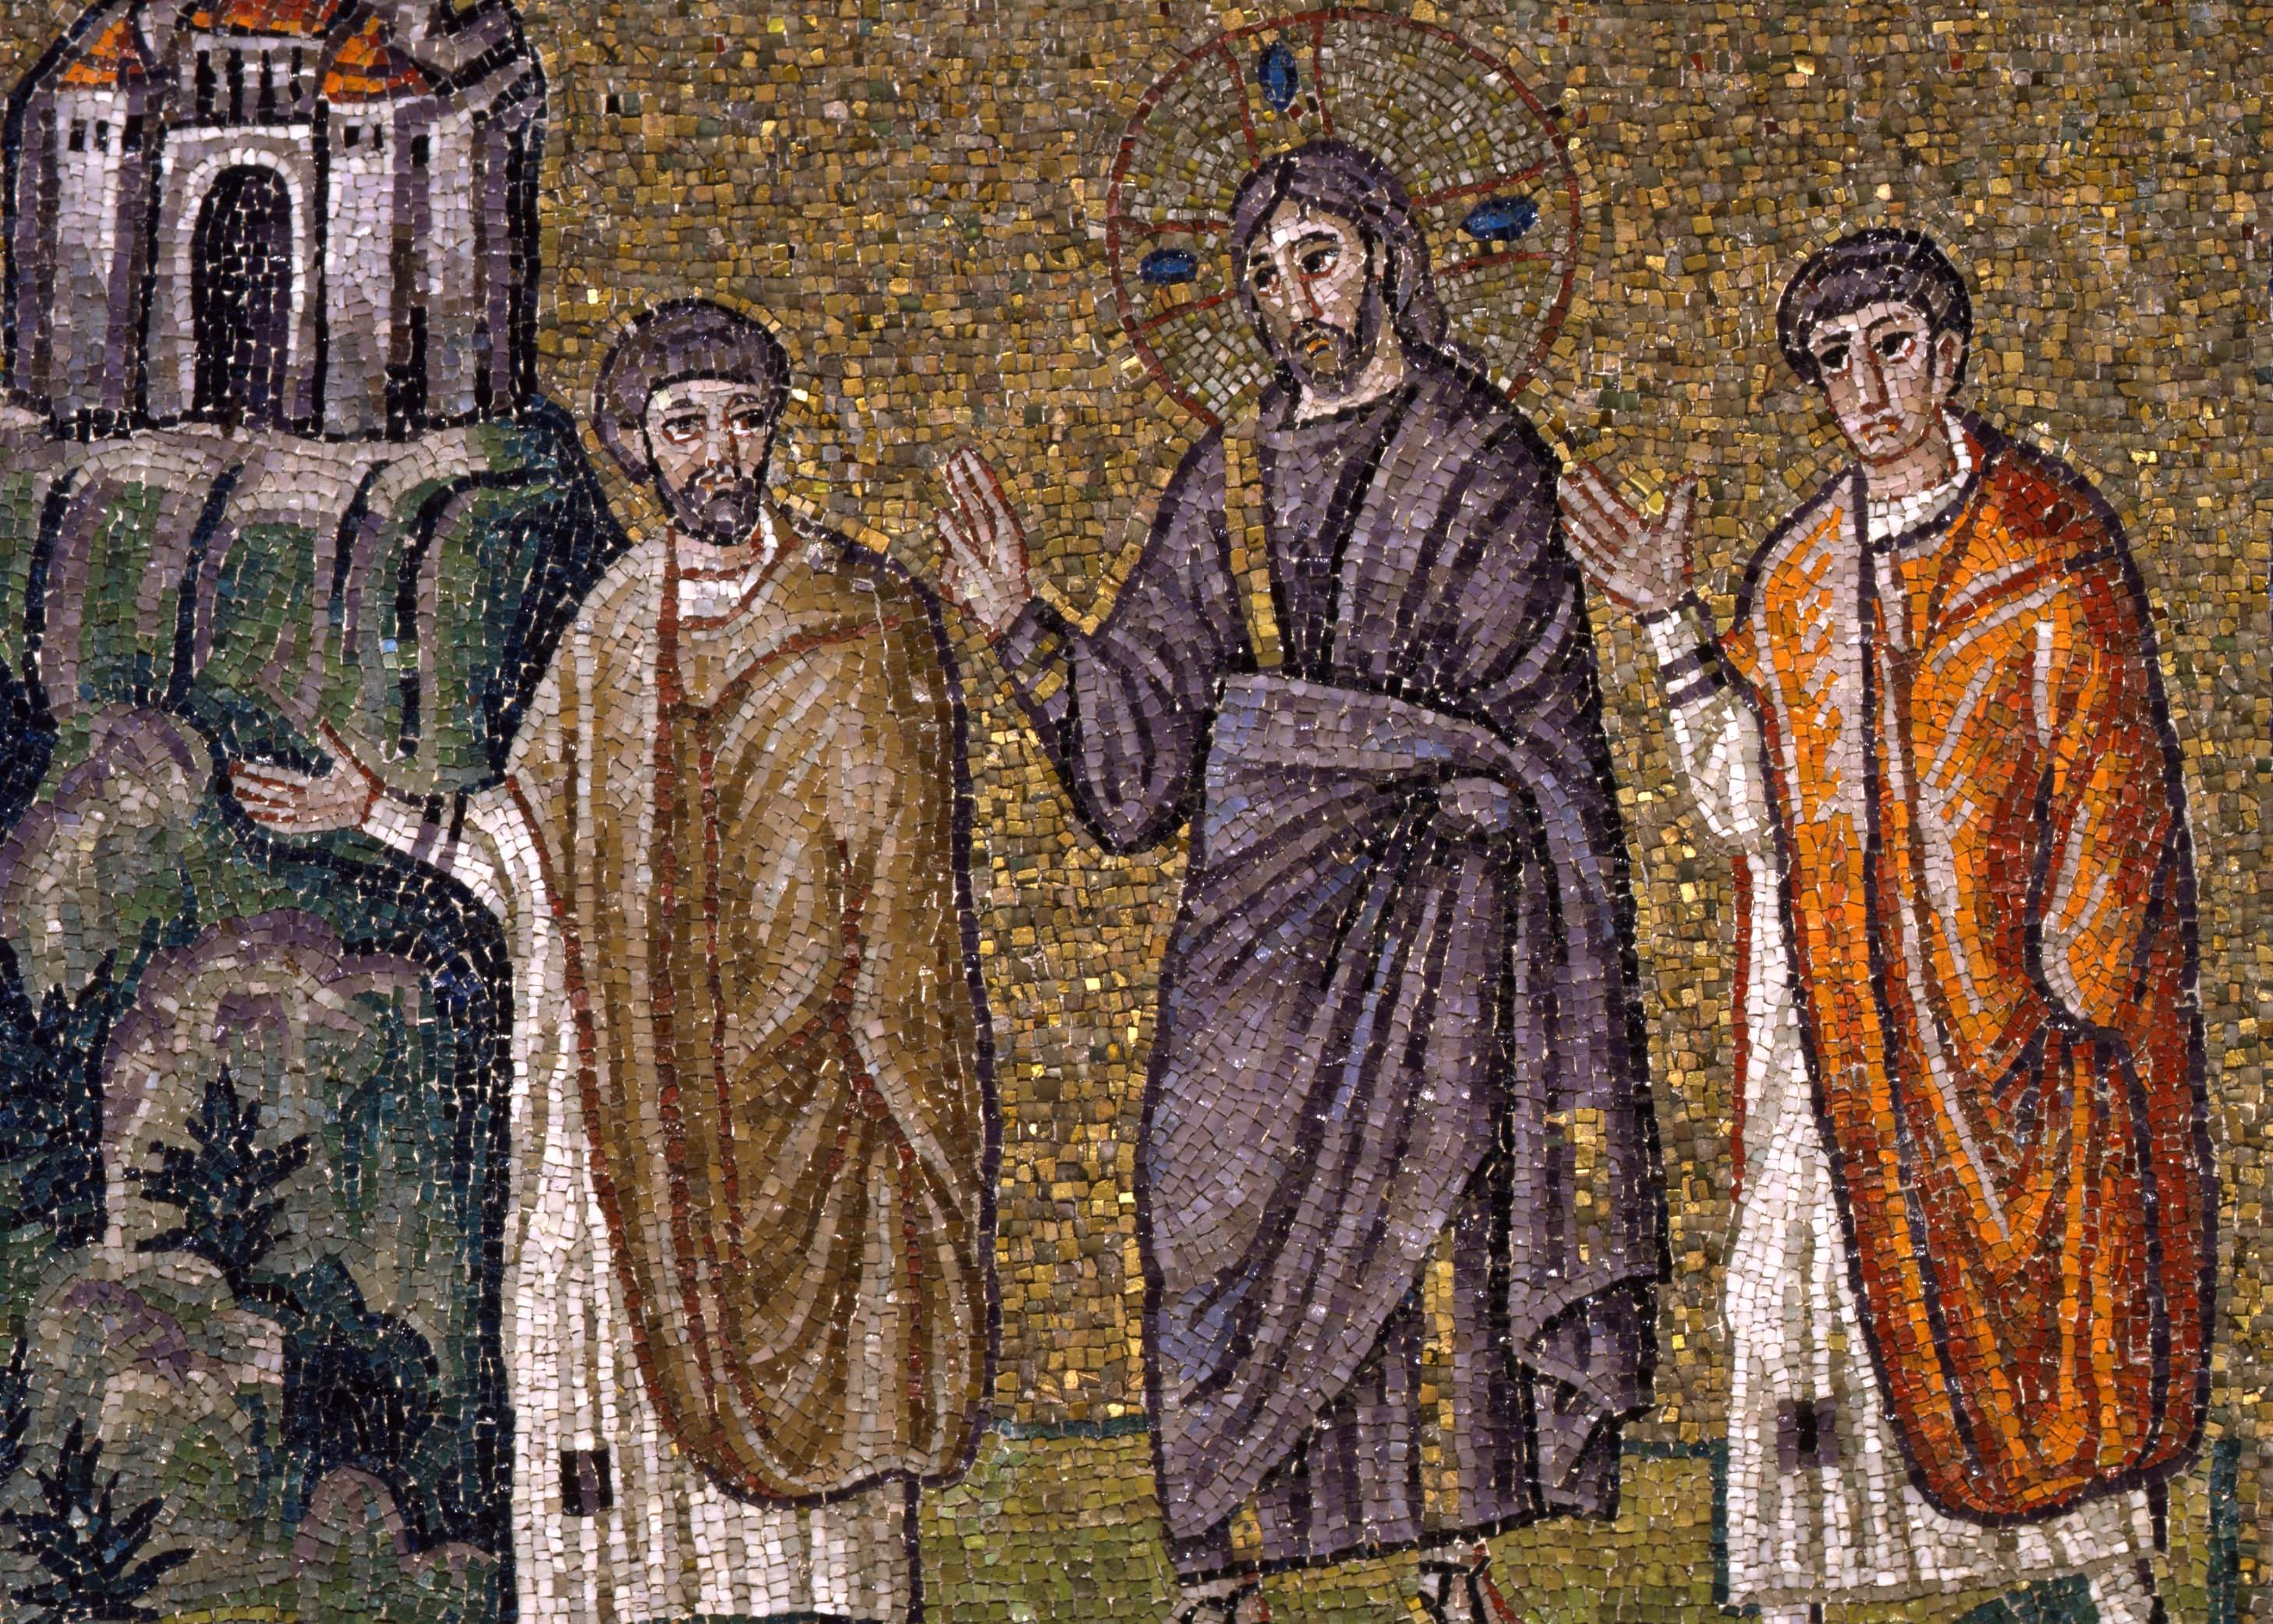
\includegraphics[width=8cm]{emmaus.jpg}
%\end{center}

\vfill

\begin{center}
%Ad usum et secundum consuetudines chori \guillemotright{}Conventus Choralis\guillemotleft.

%Editio Sancti Wolfgangi \annusEditionis
\end{center}

\pagebreak

\renewcommand{\headrulewidth}{0pt} % no horiz. rule at the header
\fancyhf{}
\pagestyle{fancy}

\cantusSineNeumas

\ifx\festum\undefined
\else
\pars{Oratio ante divinum Officium.}

\lettrine{{\color{red}A}}{peri,} Dómine, os meum ad benedicéndum nomen sanctum tuum:
munda quoque cor meum ab ómnibus vanis, pervérsis, et aliénis
cogitatiónibus:
intelléctum illúmina, afféctum inflámma,
ut digne, atténte ac devóte hoc Offícium recitáre váleam,
et exaudíri mérear ante conspéctum Divínæ Maiestátis tuæ.
Per Christum, Dóminum nostrum.
\Rbardot{} Amen.

Dómine, in unióne illíus divínæ intentiónis,
qua ipse in terris laudes Deo persolvísti,
has tibi Horas \rubricatum{(vel \textnormal{hanc tibi Horam})} persólvo.

%\trOratioAnteOfficium

\vfill

\pars{Oratio post divinum Officium.}

\rubrica{
  Orationem sequentem devote post Officium recitantibus
  Leo Papa X. defectus, et culpas in eo persolvendo ex humana
  fragilitate contractas, indulsit, et dicitur flexis genibus.
}

\lettrine{{\color{red}S}}{acrosánctæ} et indivíduæ Trinitáti,
crucifíxi Dómini nostri Iesu Christi humanitáti,
beatíssimæ et gloriosíssimæ sempérque Vírginis Maríæ
fecúndæ integritáti, 
et ómnium Sanctórum universitáti
sit sempitérna laus, honor, virtus et glória
ab omni creatúra,
nobísque remíssio ómnium peccatórum,
per infiníta sǽcula sæculórum.
\Rbardot{} Amen.

\noindent \Vbardot{} Beáta víscera Maríæ Virginis, quæ portavérunt
ætérni Patris Fílium.\\
\Rbardot{} Et beáta úbera, quæ lactavérunt Christum Dominum.

\rubrica{Et dicitur secreto \textnormal{Pater noster.} et \textnormal{Ave María.}}

%\trOratioPostOfficium

\vfill

\hora{Ad I. Vesperas.} %%%%%%%%%%%%%%%%%%%%%%%%%%%%%%%%%%%%%%%%%%%%%%%%%%%%%
%\sideThumbs{I. Vesperæ}

\vspace{0.5cm}
\grechangedim{interwordspacetext}{0.18 cm plus 0.15 cm minus 0.05 cm}{scalable}%
\ifx\festum\undefined
\cuminitiali{}{temporalia/deusinadiutorium-alter.gtex}
\else
\cuminitiali{}{temporalia/deusinadiutorium-solemnis.gtex}
\fi
\grechangedim{interwordspacetext}{0.22 cm plus 0.15 cm minus 0.05 cm}{scalable}%

\vfill
\pagebreak

\pars{Psalmus 1.} \scriptura{Io. 21, 17; \textbf{H283}}

\vspace{-0.4cm}

\antiphona{\textit{IV A}}{temporalia/ant-petreamasme.gtex}

\scriptura{Psalmus 112.}

\initiumpsalmi{temporalia/ps112-initium-iv-A-auto.gtex}

%\psalmusEtTranslatioT{temporalia/ps112ivA-comb.tex}{10cm}
\input{temporalia/ps112ivA.tex} \Abardot{}

\vspace{-1cm}

\vfill
\pagebreak

\pars{Psalmus 2.} \scriptura{2 Cor. 12, 9; \textbf{H288}}

\vspace{-0.4cm}

\antiphona{VIII G}{temporalia/ant-libentergloriabor.gtex}

\scriptura{Psalmus 116.}

\initiumpsalmi{temporalia/ps116-initium-viii-G-auto.gtex}

%\psalmusEtTranslatioT{temporalia/ps116-comb.tex}{10cm}
\input{temporalia/ps116.tex} \Abardot{}

\vfill
\pagebreak

\pars{Psalmus 3.} \scriptura{Ac. 12, 8; \textbf{H281}}

\vspace{-0.4cm}

\antiphona{VIII a}{temporalia/ant-dixitangelusadpetrum.gtex}

\scriptura{Psalmus 145.}

\initiumpsalmi{temporalia/ps145-initium-viii-A-auto.gtex}

%\psalmusEtTranslatioT{temporalia/ps145-comb.tex}{10cm}
\input{temporalia/ps145.tex} \Abardot{}

\vfill
\pagebreak

\pars{Psalmus 4.} \scriptura{2 Cor. 11, 32.33; \textbf{H289}}

\vspace{-6mm}

\antiphona{VIII G}{temporalia/ant-damascipraepositus.gtex}

\vspace{-4mm}

\scriptura{Psalmus 146.}

\vspace{-1.5mm}

\initiumpsalmi{temporalia/ps146-initium-viii-g-auto.gtex}

\vspace{-1.5mm}

%\psalmusEtTranslatioT{temporalia/ps146-comb.tex}{10cm}
\input{temporalia/ps146.tex} \Abardot{}

\vfill
\pagebreak

\pars{Psalmus 5.} \scriptura{Ac. 12, 11; \textbf{H281}}

\vspace{-0.4cm}

\antiphona{VII c\textsuperscript{2}}{temporalia/ant-misitdominus.gtex}

\scriptura{Psalmus 147.}

\initiumpsalmi{temporalia/ps147-initium-vii-c2-auto.gtex}

%\psalmusEtTranslatioT{temporalia/ps147-comb.tex}{10cm}
\input{temporalia/ps147.tex} \Abardot{}

\vfill
\pagebreak

\pars{Capitulum.} \scriptura{Ac. 12, 1-3}

\grechangedim{interwordspacetext}{0.12 cm plus 0.15 cm minus 0.05 cm}{scalable}%
\cuminitiali{}{temporalia/capitulum-MisitHerodes.gtex}
\grechangedim{interwordspacetext}{0.22 cm plus 0.15 cm minus 0.05 cm}{scalable}

% preklad Jeruz. bible
%\trCapituliI

\vfill

\ifx\festum\undefined
\pars{Responsorium breve.} \scriptura{Ps. 18, 5}

\cuminitiali{VI}{temporalia/resp-inomnemterram.gtex}
\else
\pars{Responsorium.} \scriptura{\Rbardot{} Mt. 16, 19 \Vbardot{} ibid.; \textbf{H282}}

\cuminitiali{VIII}{temporalia/resp-tuespastorovium-CROCHU.gtex}
\fi

%\trResp

\vfill
\pagebreak

\pars{Hymnus}

\cuminitiali{I}{temporalia/hym-AureaLuce.gtex}
\vspace{-3mm}
%\input{hym-AureaLuce-bohtext.tex}

\vfill
%\pagebreak

\pars{Versus.} \scriptura{Ps. 18, 5}

% Versus. %%%
\sineinitiali{temporalia/versus-inomnem.gtex}

%\noindent \trVersus

\vfill
\pagebreak

\pars{Canticum B. Mariæ V.} \scriptura{Ac. 9, 10.11.15}

\vspace{-3mm}

{
\grechangedim{interwordspacetext}{0.18 cm plus 0.15 cm minus 0.05 cm}{scalable}%
\antiphona{VII a}{temporalia/ant-vadeanania.gtex}
\grechangedim{interwordspacetext}{0.22 cm plus 0.15 cm minus 0.05 cm}{scalable}%
}

%\trAntIMagnificat

%\vspace{-2mm}

\scriptura{Lc. 1, 46-55}

%\vspace{-2mm}

\cantusSineNeumas
\initiumpsalmi{temporalia/magnificat-initium-viisoll-a.gtex}

%\psalmusEtTranslatioT{temporalia/magnificat-I-comb.tex}{10.2cm}
\input{temporalia/magnificat-I.tex} \Abardot{}

%\vspace{-1cm}

\vfill
\pagebreak

%\sideThumbs{{\scriptsize{}Fine horarum}}

\anteOrationem

\pagebreak

% Oratio. %%%
\cuminitiali{}{temporalia/oratio.gtex}

\vspace{-1mm}
%\trOrationisI

\vfill

\rubrica{Hebdomadarius dicit iterum Dominus vobiscum, vel cantor dicit:}

\vspace{2mm}

\sineinitiali{temporalia/domineexaudi.gtex}

\rubrica{Postea cantatur a cantore:}

\vspace{2mm}

\ifx\festum\undefined
\cuminitiali{II}{temporalia/benedicamus-semiduplex-vesp.gtex}
\else
\cuminitiali{II}{temporalia/benedicamus-solemnism-1vesp.gtex}
\fi

\vspace{1mm}

\vfill
\pagebreak
\fi

\hora{Ad Matutinum.} %%%%%%%%%%%%%%%%%%%%%%%%%%%%%%%%%%%%%%%%%%%%%%%%%%%%%
%\sideThumbs{Matutinum}

\vspace{2mm}

\cuminitiali{}{temporalia/dominelabiamea.gtex}

\vspace{2mm}

\pars{Invitatorium.} \scriptura{Cantor; \textbf{H443}}

\vspace{-6mm}

\antiphona{III}{temporalia/inv-regemapostolorum.gtex}

\vfill
\pagebreak

\pars{Hymnus.}

\cuminitiali{IV}{temporalia/hym-FelixPerOmnes.gtex}
\vspace{-3mm}
%\input{hym-FelixPerOmnes-bohtext.tex}

\vfill
\pagebreak

\subhora{In I. Nocturno}

\pars{Psalmus 1.} \scriptura{Ps. 18, 5; \textbf{H360}}

\vspace{-4mm}

\antiphona{II D}{temporalia/ant-inomnemterram-FKP.gtex}

%\vspace{-5mm}

\scriptura{Ps. 18}

%\vspace{-2mm}

\initiumpsalmi{temporalia/ps18-initium-ii-D-auto.gtex}

%\psalmusEtTranslatioT{temporalia/ps18-comb.tex}{10cm}
\input{temporalia/ps18.tex}

\vfill

\antiphona{}{temporalia/ant-inomnemterram-FKP.gtex}

\vfill
\pagebreak

\pars{Psalmus 2.} \scriptura{Ps. 33, 18; \textbf{H360}}

\vspace{-4mm}

\antiphona{VII c\textsuperscript{2}}{temporalia/ant-clamaveruntiusti-FKP.gtex}

%\vspace{-5mm}

\scriptura{Ps. 33}

\initiumpsalmi{temporalia/ps33-initium-vii-c2-auto.gtex}

%\psalmusEtTranslatioT{temporalia/ps33-comb.tex}{10cm}
\input{temporalia/ps33.tex}

\vfill

\antiphona{}{temporalia/ant-clamaveruntiusti-FKP.gtex}

\vfill
\pagebreak

\pars{Psalmus 3.} \scriptura{Ps. 44, 17.18; \textbf{H360}}

\vspace{-4mm}

\antiphona{VIII a}{temporalia/ant-constitueseosprincipes-FKP.gtex}

%\vspace{-2mm}

\scriptura{Ps. 44}

%\vspace{-2mm}

\initiumpsalmi{temporalia/ps44-initium-viii-A-auto.gtex}

%\psalmusEtTranslatioT{temporalia/ps44-comb.tex}{10cm}
\input{temporalia/ps44.tex}

\vfill

\antiphona{}{temporalia/ant-constitueseosprincipes-FKP.gtex}

\vfill
\pagebreak

\pars{Versus.} \scriptura{Ps. 18, 5}

% Versus. %%%
\sineinitiali{temporalia/versus-inomnem-communis.gtex}

\vspace{5mm}

\sineinitiali{temporalia/oratiodominica-mat.gtex}

\vspace{5mm}

\pars{Absolutio.}

\cuminitiali{}{temporalia/absolutio-exaudi.gtex}

\vfill
\pagebreak

\cuminitiali{}{temporalia/benedictio-solemn-benedictione.gtex}

\vspace{7mm}

\lectioi

\noindent \Vbardot{} Tu autem, Dómine, miserére nobis.
\noindent \Rbardot{} Deo grátias.

\vfill
\pagebreak

\pars{Responsorium 1.} \scriptura{\Rbardot{} Mt. 16, 19 \Vbardot{} ibid; \textbf{H280}}

\vspace{-5mm}

\responsorium{VII}{temporalia/resp-simonpetre-CROCHU.gtex}{}

\vfill
\pagebreak

\cuminitiali{}{temporalia/benedictio-solemn-unigenitus.gtex}

\vspace{7mm}

\lectioii

\noindent \Vbardot{} Tu autem, Dómine, miserére nobis.
\noindent \Rbardot{} Deo grátias.

\vfill
\pagebreak

\pars{Responsorium 2.} \scriptura{\Rbardot{} Io. 21, 15.17 \Vbardot{} Mt. 26, 35; \textbf{H280}}

\vspace{-5mm}

\responsorium{VI}{temporalia/resp-sidiligisme-CROCHU.gtex}{}

\vfill
\pagebreak

\cuminitiali{}{temporalia/benedictio-solemn-spiritus.gtex}

\vspace{7mm}

\lectioiii

\noindent \Vbardot{} Tu autem, Dómine, miserére nobis.
\noindent \Rbardot{} Deo grátias.

\vfill
\pagebreak

\pars{Responsorium 3.} \scriptura{\Rbardot{} Mt. 16, 18.19 \Vbardot{} ibid; \textbf{H280}}

\vspace{-5mm}

\responsorium{VII}{temporalia/resp-tuespetrus-CROCHU.gtex}{}

\vfill
\pagebreak

\subhora{In II. Nocturno}

\pars{Psalmus 4.} \scriptura{Ps. 46, 10; \textbf{H361}}

\vspace{-4mm}

\antiphona{VIII G}{temporalia/ant-principespopulorum-FKP.gtex}

\scriptura{Ps. 46}

%\vspace{-2mm}

\initiumpsalmi{temporalia/ps46-initium-viii-G-auto.gtex}

%\psalmusEtTranslatioT{temporalia/ps46-comb.tex}{10cm}
\input{temporalia/ps46.tex} \Abardot{}

\vfill
\pagebreak

\pars{Psalmus 5.} \scriptura{Ps. 60, 6; \textbf{H361}}

\vspace{-4mm}

\antiphona{VIII G}{temporalia/ant-dedistihereditatem-FKP.gtex}

%\vspace{-4mm}

\scriptura{Ps. 60}

%\vspace{-2mm}

\initiumpsalmi{temporalia/ps60-initium-viii-G-auto.gtex}

%\vspace{-1.5mm}

%\psalmusEtTranslatioT{temporalia/ps60-comb.tex}{10cm}
\input{temporalia/ps60.tex} \Abardot{}

\vspace{-1cm}

\vfill
\pagebreak

\pars{Psalmus 6.} \scriptura{Ps. 63, 10; \textbf{H361}}

\vspace{-4mm}

\antiphona{VIII G}{temporalia/ant-anuntiaverunt-FKP.gtex}

%\vspace{-5mm}

\scriptura{Ps. 63}

\initiumpsalmi{temporalia/ps63-initium-viii-G-auto.gtex}

%\psalmusEtTranslatioT{temporalia/ps63-comb.tex}{10cm}
\input{temporalia/ps63.tex} \Abardot{}

%\vfill

%\antiphona{}{temporalia/ant-anuntiaverunt-FKP.gtex}

\vfill
\pagebreak

\pars{Versus.} \scriptura{Ps. 44, 17-18}

% Versus. %%%
\sineinitiali{temporalia/versus-constitues.gtex}

\vspace{5mm}

\sineinitiali{temporalia/oratiodominica-mat.gtex}

\vspace{5mm}

\pars{Absolutio.}

\cuminitiali{}{temporalia/absolutio-ipsius.gtex}

\vfill
\pagebreak

\cuminitiali{}{temporalia/benedictio-solemn-deus.gtex}

\vspace{7mm}

\lectioiv

\noindent \Vbardot{} Tu autem, Dómine, miserére nobis.
\noindent \Rbardot{} Deo grátias.

\vfill
\pagebreak

\pars{Responsorium 4.} \scriptura{\Rbardot{} Mt. 14, 28.31 \Vbardot{} ibid. 14, 30; \textbf{H281}}

\vspace{-5mm}

\responsorium{VIII}{temporalia/resp-dominesitues-CROCHU.gtex}{}

\vfill
\pagebreak

\cuminitiali{}{temporalia/benedictio-solemn-christus.gtex}

\vspace{7mm}

\lectiov

\noindent \Vbardot{} Tu autem, Dómine, miserére nobis.
\noindent \Rbardot{} Deo grátias.

\vfill
\pagebreak

\pars{Responsorium 5.} \scriptura{\Rbardot{} Ac. 12, 7.8 \Vbardot{} ibid. 12, 7; \textbf{H281}}

\vspace{-5mm}

\responsorium{VII}{temporalia/resp-surgepetre-CROCHU.gtex}{}

\vfill
\pagebreak

\cuminitiali{}{temporalia/benedictio-solemn-ignem.gtex}

\vspace{7mm}

\lectiovi

\noindent \Vbardot{} Tu autem, Dómine, miserére nobis.
\noindent \Rbardot{} Deo grátias.

\vfill
\pagebreak

\pars{Responsorium 6.} \scriptura{\Rbardot{} Mt. 16, 19 \Vbardot{} ibid.; \textbf{H282}}

\vspace{-5mm}

\responsorium{VIII}{temporalia/resp-tuespastorovium-CROCHU.gtex}{}

\vfill
\pagebreak

\subhora{In III. Nocturno}

\pars{Psalmus 7.} \scriptura{Ps. 74, 11; \textbf{H361}}

\vspace{-4mm}

\antiphona{VI F}{temporalia/ant-exaltabunturcornuaiusti-FKP.gtex}

%\vspace{-4mm}

\scriptura{Ps. 74}

%\vspace{-2mm}

\initiumpsalmi{temporalia/ps74-initium-vi-F-auto.gtex}

%\psalmusEtTranslatioT{temporalia/ps74-comb.tex}{10cm}
\input{temporalia/ps74.tex} \Abardot{}

\vfill
\pagebreak

\pars{Psalmus 8.} \scriptura{Ps. 96, 11; \textbf{H361}}

\vspace{-4mm}

\antiphona{VI F}{temporalia/ant-luxortaestiustis-FKP.gtex}

%\vspace{-3mm}

\scriptura{Ps. 96}

%\vspace{-2mm}

\initiumpsalmi{temporalia/ps96-initium-vi-F-auto.gtex}

%\vspace{-1mm}

%\psalmusEtTranslatioT{temporalia/ps96-comb.tex}{10cm}
\input{temporalia/ps96.tex} \Abardot{}

\vfill
\pagebreak

\pars{Psalmus 9.} \scriptura{Ps. 98, 7; \textbf{H361}}

\vspace{-4mm}

\antiphona{\textit{IV A}}{temporalia/ant-custodiebant-FKP.gtex}

%\vspace{-3mm}

\scriptura{Ps. 98}

%\vspace{-3mm}

\initiumpsalmi{temporalia/ps98-initium-iv-A-auto.gtex}

%\vspace{-1.5mm}

%\psalmusEtTranslatioT{temporalia/ps98-comb.tex}{10cm}
\input{temporalia/ps98.tex} \Abardot{}

\vfill
\pagebreak

\pars{Versus.} \scriptura{Ps. 138, 17}

% Versus. %%%
\sineinitiali{temporalia/versus-nimis.gtex}

\vspace{5mm}

\sineinitiali{temporalia/oratiodominica-mat.gtex}

\vspace{5mm}

\pars{Absolutio.}

\cuminitiali{}{temporalia/absolutio-avinculis.gtex}

\vfill
\pagebreak

\cuminitiali{}{temporalia/benedictio-solemn-evangelica.gtex}

\vspace{7mm}

\lectiovii

\noindent \Vbardot{} Tu autem, Dómine, miserére nobis.
\noindent \Rbardot{} Deo grátias.

\vfill
\pagebreak

\pars{Responsorium 7.} \scriptura{\Rbardot{} Lc. 22, 32 \Vbardot{} Mt. 16, 17; \textbf{H282}}

\vspace{-5mm}

\responsorium{III}{temporalia/resp-egoproterogavi-CROCHU.gtex}{}

\vfill
\pagebreak

\cuminitiali{}{temporalia/benedictio-solemn-quorum.gtex}

\vspace{7mm}

\lectioviii

\noindent \Vbardot{} Tu autem, Dómine, miserére nobis.
\noindent \Rbardot{} Deo grátias.

\vfill
\pagebreak

\pars{Responsorium 8.} \scriptura{\Rbardot{} Mt. 16, 13.16.18 \Vbardot{} ibid. 16, 17; \textbf{H282}}

\vspace{-5mm}

\responsorium{I}{temporalia/resp-quemdicunthomines-CROCHU.gtex}{}

\vfill
\pagebreak

\cuminitiali{}{temporalia/benedictio-solemn-adsocietatem.gtex}

\vspace{7mm}

\lectioix

\noindent \Vbardot{} Tu autem, Dómine, miserére nobis.
\noindent \Rbardot{} Deo grátias.

\vfill
\pagebreak

% Te Deum

%\pars{Hymnus Ambrosianus}

\vspace{-5mm}

\ifx\solemnis\undefined
\ifx\aequus\undefined
{
\pars{Hymnus Ambrosianus} \scriptura{Alio modo, iuxta morem Romanum}

\vspace{-2mm}

\grechangedim{interwordspacetext}{0.26 cm plus 0.15 cm minus 0.05 cm}{scalable}%
\cuminitiali{III}{temporalia/tedeum-romanum-gn.gtex}
\grechangedim{interwordspacetext}{0.22 cm plus 0.15 cm minus 0.05 cm}{scalable}%
}
\else
{
\pars{Hymnus Ambrosianus} \scriptura{Tonus Simplex}

\vspace{-2mm}

\grechangedim{interwordspacetext}{0.30 cm plus 0.15 cm minus 0.05 cm}{scalable}%
\cuminitiali{III}{temporalia/tedeum-simplex-gn.gtex}
\grechangedim{interwordspacetext}{0.22 cm plus 0.15 cm minus 0.05 cm}{scalable}%
}
\fi
\else
{
\pars{Hymnus Ambrosianus} \scriptura{Tonus Solemnis}

\vspace{-2mm}

\grechangedim{interwordspacetext}{0.26 cm plus 0.15 cm minus 0.05 cm}{scalable}%
\cuminitiali{III}{temporalia/tedeum-solemnis-gn.gtex}
\grechangedim{interwordspacetext}{0.22 cm plus 0.15 cm minus 0.05 cm}{scalable}%
}
\fi

\vfill
\pagebreak

\rubrica{Reliqua omittuntur, nisi Laudes separandæ sint.}

\sineinitiali{temporalia/domineexaudi.gtex}

\vfill

\pars{Oratio.}

\cuminitiali{}{temporalia/oratio.gtex}

\vfill

\noindent \Vbardot{} Dómine, exáudi oratiónem meam.
\Rbardot{} Et clamor meus ad te véniat.

\vfill

% Nocturnale Romanum 2002, p. LXXVI Benedicamus Domino seems to match
% the one from Solemn Laudes.
\cuminitiali{V}{temporalia/benedicamus-solemnis-laud.gtex}

\vfill

\noindent \Vbardot{} Fidélium ánimæ per misericórdiam Dei requiéscant in pace.
\Rbardot{} Amen.

\vfill
\pagebreak

\hora{Ad Laudes.} %%%%%%%%%%%%%%%%%%%%%%%%%%%%%%%%%%%%%%%%%%%%%%%%%%%%%
%\sideThumbs{Laudes}

\cantusSineNeumas

\vspace{0.5cm}
\grechangedim{interwordspacetext}{0.18 cm plus 0.15 cm minus 0.05 cm}{scalable}%
\ifx\festumveldominica\undefined
\cuminitiali{}{temporalia/deusinadiutorium-communis.gtex}
\else
\cuminitiali{}{temporalia/deusinadiutorium-alter.gtex}
\fi
\grechangedim{interwordspacetext}{0.22 cm plus 0.15 cm minus 0.05 cm}{scalable}%

\vfill
%\pagebreak

\pars{Psalmus 1.} \scriptura{1 Cor. 3, 6; \textbf{H288}}

\vspace{-6mm}

\antiphona{VIII G}{temporalia/ant-egoplantaviapollorigavit.gtex}

\vspace{-2mm}

\scriptura{Psalmus 92.}

\vspace{-1mm}

\initiumpsalmi{temporalia/ps92-initium-viii-g-auto.gtex}

%\psalmusEtTranslatioT{temporalia/ps92-comb.tex}{10cm}
\input{temporalia/ps92.tex} \Abardot{}

\vfill
\pagebreak

\pars{Psalmus 2.} \scriptura{Mt. 16, 18; \textbf{H283}}

\vspace{-0.4cm}

\antiphona{VII c}{temporalia/ant-tuespetrus.gtex}

\scriptura{Psalmus 99.}

\initiumpsalmi{temporalia/ps99-initium-vii-c-auto.gtex}

%\psalmusEtTranslatioT{temporalia/ps99-comb.tex}{10cm}
\input{temporalia/ps99.tex} \Abardot{}

\vfill
\pagebreak

\pars{Psalmus 3.} \scriptura{\textbf{H288}}

\vspace{-0.4cm}

\antiphona{VIII G}{temporalia/ant-sanctepauleapostole.gtex}

\scriptura{Psalmus 62.}

\initiumpsalmi{temporalia/ps62-initium-viii-G-auto.gtex}

%\psalmusEtTranslatioT{temporalia/ps62-comb.tex}{10cm}
\input{temporalia/ps62.tex} \Abardot{}

\vfill
\pagebreak

\pars{Psalmus 4.} \scriptura{Lc. 22, 32; \textbf{H283}}

\vspace{-0.4cm}

\antiphona{VIII G}{temporalia/ant-egoproterogavi.gtex}

\scriptura{Canticum trium puerorum, Dan. 3, 57-88 et 56}

\initiumpsalmi{temporalia/dan3-initium-viii-G-auto.gtex}

%\psalmusEtTranslatioT{temporalia/dan3-comb.tex}{10cm}
\input{temporalia/dan3.tex}

\rubrica{Hic non dicitur Gloria Patri, neque Amen.}

\vfill

\vspace{-6mm}

\antiphona{}{temporalia/ant-egoproterogavi.gtex} % repeat the antiphon - new page

\vfill
\pagebreak

\pars{Psalmus 5.} \scriptura{1 Cor. 15, 10; \textbf{H288}}

\vspace{-0.4cm}

\antiphona{\textit{IV A*}}{temporalia/ant-gratiadeiinme.gtex}

\scriptura{Psalmus 148.}

\initiumpsalmi{temporalia/ps148-initium-iv-A_-auto.gtex}

%\psalmusEtTranslatioT{temporalia/ps148-comb.tex}{10cm}
\input{temporalia/ps148.tex}

\rubrica{Hic non dicitur Gloria Patri.}

\vfill
\pagebreak

%
\scriptura{Psalmus 149.}

\initiumpsalmi{temporalia/ps149-initium-iv-A_-auto.gtex}

%\psalmusEtTranslatioT{temporalia/ps149-comb.tex}{10cm}
\input{temporalia/ps149.tex}

\rubrica{Hic non dicitur Gloria Patri.}

\vfill
\pagebreak

%
\scriptura{Psalmus 150.}

\initiumpsalmi{temporalia/ps150-initium-iv-A_-auto.gtex}

%\psalmusEtTranslatioT{temporalia/ps150-comb.tex}{10cm}
\input{temporalia/ps150.tex}

\vfill

\vspace{-6mm}

\antiphona{}{temporalia/ant-gratiadeiinme.gtex} % repeat the antiphon - new page

\vfill
\pagebreak

\pars{Capitulum.} \scriptura{Ac. 12, 1-3}

\grechangedim{interwordspacetext}{0.12 cm plus 0.15 cm minus 0.05 cm}{scalable}%
\cuminitiali{}{temporalia/capitulum-MisitHerodes.gtex}
\grechangedim{interwordspacetext}{0.22 cm plus 0.15 cm minus 0.05 cm}{scalable}

% preklad Jeruz. bible
%\trCapituliI

\vfill

\pars{Responsorium breve.} \scriptura{Ps. 18, 5}

\cuminitiali{VI}{temporalia/resp-inomnemterram.gtex}

%\trResp

\vfill
\pagebreak

\pars{Hymnus}

\ifx\festum\undefined
\grechangedim{interwordspacetext}{0.16 cm plus 0.15 cm minus 0.05 cm}{scalable}%
\cuminitiali{IV}{temporalia/hym-ApostolorumPassio.gtex}
\grechangedim{interwordspacetext}{0.22 cm plus 0.15 cm minus 0.05 cm}{scalable}%
\vspace{-3mm}
%\input{hym-ApostolorumPassio-bohtext.tex}
\vfill
\pagebreak
\else
\cuminitiali{IV}{temporalia/hym-JamBonePastor.gtex}
\vspace{-3mm}
%\input{hym-JamBonePastor-bohtext.tex}
\vfill
%\pagebreak
\fi

\pars{Versus.} \scriptura{Ps. 63, 10}

% Versus. %%%
\ifx\festum\undefined
\sineinitiali{temporalia/versus-annuntiaverunt-communis.gtex}
\else
\sineinitiali{temporalia/versus-annuntiaverunt.gtex}
\fi

%\noindent \trVersus

\vfill
\pagebreak

\pars{Canticum Zachariæ.} \scriptura{\textbf{H284}}

\vspace{-4mm}

{
\grechangedim{interwordspacetext}{0.18 cm plus 0.15 cm minus 0.05 cm}{scalable}%
\antiphona{VI F}{temporalia/ant-gloriosiprincipes.gtex}
\grechangedim{interwordspacetext}{0.22 cm plus 0.15 cm minus 0.05 cm}{scalable}%
}

%\trAntIMagnificat

%\vspace{-2mm}

\scriptura{Lc. 1, 68-79}

\vspace{-1mm}

\cantusSineNeumas
\ifx\solemnis\undefined
\initiumpsalmi{temporalia/benedictus-initium-vi-F-auto.gtex}

%\vspace{-1.5mm}

%\psalmusEtTranslatioT{temporalia/benedictus-II-comb.tex}{10.2cm}
\input{temporalia/benedictus-II.tex} \Abardot{}
\else
\initiumpsalmi{temporalia/benedictus-initium-visoll-F-auto.gtex}

%\vspace{-1.5mm}

%\psalmusEtTranslatioT{temporalia/benedictus-I-comb.tex}{10.2cm}
\input{temporalia/benedictus-I.tex} \Abardot{}
\fi

\vspace{-1cm}

\vfill
\pagebreak

%\sideThumbs{{\scriptsize{}Fine horarum}}

\anteOrationem

\pagebreak

% Oratio. %%%
\cuminitiali{}{temporalia/oratio.gtex}

\vspace{-1mm}
%\trOrationisI

\vfill

\rubrica{Hebdomadarius dicit iterum Dominus vobiscum, vel cantor dicit:}

\vspace{2mm}

\sineinitiali{temporalia/domineexaudi.gtex}

\rubrica{Postea cantatur a cantore:}

\vspace{2mm}

\ifx\festum\undefined
\ifx\octava\undefined
\cuminitiali{I}{temporalia/benedicamus-semiduplex-laud.gtex}
\else
\cuminitiali{VIII}{temporalia/benedicamus-duplexmajus-laudes.gtex}
\fi
\else
\cuminitiali{II}{temporalia/benedicamus-solemnism-laud.gtex}
\fi

\vspace{1mm}

\vfill
\pagebreak

\ifx\sabbatoveloctava\undefined
\ifx\festumveldominica\undefined
\hora{Ad Vesperas.} %%%%%%%%%%%%%%%%%%%%%%%%%%%%%%%%%%%%%%%%%%%%%%%%%%%%%
%\sideThumbs{Vesperæ}
\else
\hora{Ad II. Vesperas.} %%%%%%%%%%%%%%%%%%%%%%%%%%%%%%%%%%%%%%%%%%%%%%%%%%%%%
%\sideThumbs{II. Vesperæ}
\fi

\cantusSineNeumas

%\vspace{-2mm}
\grechangedim{interwordspacetext}{0.18 cm plus 0.15 cm minus 0.05 cm}{scalable}%
\ifx\festumveldominica\undefined
\cuminitiali{}{temporalia/deusinadiutorium-communis.gtex}
\else
\ifx\festum\undefined
\cuminitiali{}{temporalia/deusinadiutorium-alter.gtex}
\else
\cuminitiali{}{temporalia/deusinadiutorium-solemnis.gtex}
\fi
\fi
\grechangedim{interwordspacetext}{0.22 cm plus 0.15 cm minus 0.05 cm}{scalable}%

\vfill
%\pagebreak

%\vspace{-2mm}

\pars{Psalmus 1.} \scriptura{Ac. 3, 1; \textbf{H279}}

\vspace{-0.4cm}

\antiphona{VIII G}{temporalia/ant-petrusetjoannes.gtex}

\scriptura{Psalmus 109.}

\initiumpsalmi{temporalia/ps109-initium-viii-g-auto.gtex}

%\psalmusEtTranslatioT{temporalia/ps109-comb.tex}{10cm}
\input{temporalia/ps109.tex} \Abardot{}

\vfill
\pagebreak

\pars{Psalmus 2.} \scriptura{Ac. 3, 6; \textbf{H280}}

\vspace{-0.4cm}

\antiphona{VII d}{temporalia/ant-argentumetaurum.gtex}

\scriptura{Psalmus 112.}

\initiumpsalmi{temporalia/ps112-initium-vii-d-auto.gtex}

%\psalmusEtTranslatioT{temporalia/ps112-comb.tex}{10cm}
\input{temporalia/ps112.tex} \Abardot{}

\vfill
\pagebreak

\pars{Psalmus 3.} \scriptura{Phil. 1, 1, 21; Gal. 6, 14; \textbf{H284}}

\vspace{-0.4cm}

\antiphona{I g}{temporalia/ant-mihivivere.gtex}

\scriptura{Psalmus 115.}

\initiumpsalmi{temporalia/ps115-initium-i-g-auto.gtex}

%\psalmusEtTranslatioT{temporalia/ps115-comb.tex}{10cm}
\input{temporalia/ps115.tex} \Abardot{}

\vfill
\pagebreak

\pars{Psalmus 4.} \scriptura{2 Cor. 11, 25; \textbf{H286}}

\vspace{-0.4cm}

\antiphona{VIII G}{temporalia/ant-tervirgiscaesus.gtex}

\scriptura{Psalmus 138.}

\initiumpsalmi{temporalia/ps138-initium-viii-g-auto.gtex}

%\psalmusEtTranslatioT{temporalia/ps138-comb.tex}{10cm}
\input{temporalia/ps138.tex}

\vfill

\antiphona{}{temporalia/ant-tervirgiscaesus.gtex}

\vfill
\pagebreak

\pars{Capitulum.} \scriptura{Ac. 12, 1-3}

\grechangedim{interwordspacetext}{0.12 cm plus 0.15 cm minus 0.05 cm}{scalable}%
\cuminitiali{}{temporalia/capitulum-MisitHerodes.gtex}
\grechangedim{interwordspacetext}{0.22 cm plus 0.15 cm minus 0.05 cm}{scalable}

% preklad Jeruz. bible
%\trCapituliI

\vfill

\pars{Responsorium breve.} \scriptura{Ps. 18, 5}

\cuminitiali{VI}{temporalia/resp-inomnemterram.gtex}

%\trResp

\vfill
\pagebreak

\pars{Hymnus}

\cuminitiali{IV}{temporalia/hym-ORomaFelix.gtex}
\vspace{-3mm}
%\input{hym-ORomaFelix-bohtext.tex}

\vfill
%\pagebreak

\pars{Versus.} \scriptura{Ps. 63, 10}

% Versus. %%%
\ifx\festum\undefined
\sineinitiali{temporalia/versus-annuntiaverunt-communis.gtex}
\else
\sineinitiali{temporalia/versus-annuntiaverunt.gtex}
\fi

%\noindent \trVersus

\vfill
\pagebreak

\pars{Canticum B. Mariæ V.}

\vspace{-3mm}

{
\grechangedim{interwordspacetext}{0.18 cm plus 0.15 cm minus 0.05 cm}{scalable}%
\antiphona{I D*}{temporalia/ant-hodiesimonpetrus.gtex}
\grechangedim{interwordspacetext}{0.22 cm plus 0.15 cm minus 0.05 cm}{scalable}%
}

%\trAntIMagnificat

%\vspace{-3mm}

\scriptura{Lc. 1, 46-55}

%\vspace{-2.5mm}

\cantusSineNeumas
\ifx\solemnis\undefined
\initiumpsalmi{temporalia/magnificat-initium-i-D_.gtex}

%\vspace{-1.5mm}

%\psalmusEtTranslatioT{temporalia/magnificat-III-comb.tex}{10.2cm}
\input{temporalia/magnificat-III.tex}
\else
\initiumpsalmi{temporalia/magnificat-initium-isoll-D_.gtex}

%\vspace{-1.5mm}

%\psalmusEtTranslatioT{temporalia/magnificat-II-comb.tex}{10.2cm}
\input{temporalia/magnificat-II.tex}
\fi

\vfill

{
\grechangedim{interwordspacetext}{0.18 cm plus 0.15 cm minus 0.05 cm}{scalable}%
\antiphona{}{temporalia/ant-hodiesimonpetrus.gtex}
\grechangedim{interwordspacetext}{0.22 cm plus 0.15 cm minus 0.05 cm}{scalable}%
}

\vspace{-1cm}

\vfill
\pagebreak

%\sideThumbs{{\scriptsize{}Fine horarum}}

\anteOrationem

\pagebreak

% Oratio. %%%
\cuminitiali{}{temporalia/oratio.gtex}

\vspace{-1mm}
%\trOrationisI

\vfill

\rubrica{Hebdomadarius dicit iterum Dominus vobiscum, vel cantor dicit:}

\vspace{2mm}

\sineinitiali{temporalia/domineexaudi.gtex}

\rubrica{Postea cantatur a cantore:}

\vspace{2mm}

\ifx\festum\undefined
\cuminitiali{II}{temporalia/benedicamus-semiduplex-vesp.gtex}
\else
\cuminitiali{II}{temporalia/benedicamus-solemnism-2vesp.gtex}
\fi

\vspace{1mm}
\fi

\end{document}

